\documentclass[a4paper, 12pt]{article}
% packages
\usepackage{amssymb}
\usepackage[fleqn]{mathtools}
\usepackage{tikz}
\usepackage{enumerate}
\usepackage{bussproofs}
\usepackage{xcolor}
\usepackage[margin=1.3cm]{geometry}
\usepackage{logicproof}
\usepackage{diagbox}

% augmented matrix
\makeatletter
\renewcommand*\env@matrix[1][*\c@MaxMatrixCols c]{%
\hskip -\arraycolsep
\let\@ifnextchar\new@ifnextchar
\array{#1}}
\makeatother

% ceiling / floor
\DeclarePairedDelimiter{\ceil}{\lceil}{\rceil}
\DeclarePairedDelimiter{\floor}{\lfloor}{\rfloor}

% custom commands
\newcommand{\indefint}[2]{\int #1 \, \mathrm{d}#2}
\newcommand{\defint}[4]{\int_#1^#2 #3 \, \mathrm{d}#4}
\newcommand{\dif}[2]{\frac{\mathrm{d}#1}{\mathrm{d}#2}}
\newcommand{\limit}[2]{\displaystyle{\lim_{#1 \to #2}}}
\newcommand{\summation}[3]{\sum\limits_{#1}^#2 #3}
\newcommand{\intbracket}[3]{\left[#3\right]_#1^#2}

\newcommand{\powerset}[0]{\wp}
\renewcommand{\emptyset}[0]{\varnothing}

\newcommand{\unaryproof}[2]{\AxiomC{#1} \UnaryInfC{#2} \DisplayProof}
\newcommand{\binaryproof}[3]{\AxiomC{#1} \AxiomC{#2} \BinaryInfC{#3} \DisplayProof}

% no indent
\setlength\parindent{0pt}

% reasoning proofs
\newcommand{\proofline}[3]{(#1)\ & #2 & \text{#3} \\}
\allowdisplaybreaks

% actual document
\begin{document}
    \section*{CO112 - Hardware}
        \subsection*{Prelude}
            The content discussed here is part of CO112 - Hardware (Computing MEng); taught by Bernhard Kainz, and Bjoern Schuller, in Imperial College London during the academic year 2018/19. The notes are written for my personal use, and have no guarantee of being correct (although I hope it is, for my own sake). This should be used in conjunction with the notes, and lecture slides. This course starts off fairly slow, especially if you have an idea of how logic gates work, and therefore the first parts won't be covered in much detail.
        \subsection*{Lecture 1 \hfill Notes}
            This section will be covered in less detail, as we've gone through the majority of this in much greater depth during logic. However, we will need to change the notation we use in this course from the one used in logic, from using $\land$ to $\cdot$, $\lor$ to $+$, and from $\neg$ to $^\prime$.
            \begin{center}
                \begin{tabular}{cc|c|c|c}
                    $A$ & $B$ & $A \cdot B$ (AND) & $A + B$ (OR) & $A^\prime$ (NOT) \\
                    \hline
                    0 & 0 & 0 & 0 & 1 \\
                    0 & 1 & 0 & 1 & 1 \\
                    1 & 0 & 0 & 1 & 0 \\
                    1 & 1 & 1 & 1 & 0
                \end{tabular}
            \end{center}
            The same distributivity laws apply, just like in \textbf{CO140}, as well as the simplification laws. In general, the laws should be the same as propositional logic, with the notation being slightly changed. Use 1 for $\top$, and 0 for $\bot$. We will also be using de Morgan's theorem on any number of variables (this can be proven by induction), such that $(V_1 + V_2 + V3 + ... + V_n)^\prime \equiv V_1^\prime \cdot V_2^\prime \cdot V_3^\prime \cdot ... \cdot V_n^\prime$, and the same the other way around. This can be very useful later on, as we will often use NAND / NOR gates to reduce silicon area.
        \subsection*{Lecture 2 \hfill Notes}
            The three operators covered in the first lecture can be represented by three logic gates; AND, OR, and NOT. The inverter (NOT), is represented by the circle at the end of the triangle. We can also create operations such as NAND, and NOR. Any of the first three gates can be built with just NAND gates, or just NOR gates. Let us represent $A$ NAND $B$, with $A \uparrow B$.
            \begin{itemize}
                \itemsep0em
                \item $A^\prime$ \hfill $A \uparrow A$
                \item $A \cdot B$ \hfill $(A \uparrow B)^\prime$
                    \subitem \hfill $(A \uparrow B) \uparrow (A \uparrow B)$
                \item $A + B$ \hfill $(A ^\prime \cdot B^\prime)^\prime$ (de Morgan's)
                    \subitem \hfill $A^\prime \uparrow B^\prime$
                    \subitem \hfill $(A \uparrow A) \uparrow (B \uparrow B)$
            \end{itemize}
            We also need to introduce two new gates, which are commonly used in digital logic; XOR, and XNOR. Roughly, you can use the same rules for $\neg (A \leftrightarrow B)$, and $A \leftrightarrow B$ respectively. XOR is commonly represented by $A \oplus B$ (which is much shorter than $A \cdot B^\prime + A^\prime \cdot B$), and XNOR represented by $(A \oplus B)^\prime$, instead of $A^\prime \cdot B^\prime + A \cdot B$. It has the following truth table;
            \begin{center}
                \begin{tabular}{cc|c|c}
                    $A$ & $B$ & $A \oplus B$ & $(A \oplus B)^\prime$ \\
                    \hline
                    0 & 0 & 0 & 1 \\
                    0 & 1 & 1 & 0 \\
                    1 & 0 & 1 & 0 \\
                    1 & 1 & 0 & 1
                \end{tabular}
            \end{center}
            In general, with $n$ inputs, we can have $2^n$ unique gates.
        \subsection*{Lecture 14 \hfill Panopto}
            Putting together a manual processor; generally the block diagram takes in a sequence of binary numbers, one sequence for data, and another for instructions. This will result in a binary number. Our design is based on the von Neumann architecture, which divides the processor into arithmetic units and registers, with a shared stream for data, and instructions. Our model will be based on 8 bits.
            \medskip

            Our example action is to find the average of two numbers, $A$, and $B$, such that $R = \frac{A + B}{2}$. Since we are dealing with 8 bits, $A + B < 256$.
            \begin{enumerate}[1.]
                \itemsep0em
                \item The first number is set up in input lines, and stored in register (A)
                \item The same is done for the second number, and stored in register (B)
                \item The arithmetic circuits are set to register (A) + (B).
                \item The resulting sum is put into (A)
                \item The shift circuits shift (A) one bit to the right, which is integer division by 2
                \item Result is loaded into (Res).
            \end{enumerate}
            In order to do this, we need a number of components;
            \begin{itemize}
                \item Registers
                    \begin{itemize}
                        \item store data (A), and (B)
                        \item store result (Res)
                        \item one bit for carry (C)
                        \item store instruction (IR)
                    \end{itemize}
                \item Arithmetic circuits
                    \begin{itemize}
                        \item 8-bit adder
                        \item 8-bit shifter
                    \end{itemize}
            \end{itemize}
            Note in the figure below, that the 8 means it is an 8-bit line.

            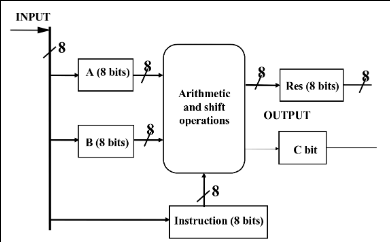
\includegraphics[]{2019-04-08-15-00-51.png}
            PANOPTO 1:21:56
            \medskip

            \begin{figure}[h!]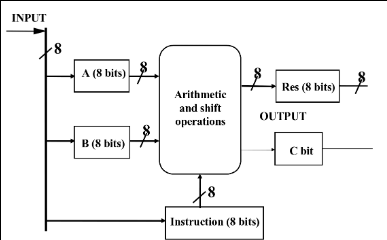
\includegraphics[width=\linewidth]{2019-04-08-20-08-22.png}\end{figure}

            For an $n$-bit ALU, there are $n + 1$ multiplexers, as the last one handles the carry bit. The $C_\text{in}$ bit for the $n^\text{th}$ multiplexer is the $C_\text{out}$ for the $(n - 1)^\text{th}$ multiplexer. The $C_\text{in}$ for the first multiplexer is 0.
        \subsection*{Notes - Lecture 14}


\end{document}
